% Created 2025-03-07 Fri 15:53
% Intended LaTeX compiler: pdflatex
\documentclass[letterpaper, 14pt]{article}
\usepackage[utf8]{inputenc}
\usepackage[T1]{fontenc}
\usepackage{graphicx}
\usepackage{longtable}
\usepackage{wrapfig}
\usepackage{rotating}
\usepackage[normalem]{ulem}
\usepackage{amsmath}
\usepackage{amssymb}
\usepackage{capt-of}
\usepackage{hyperref}
\usepackage{minted}
\usemintedstyle{manni}
\usepackage{pdfpages}
\usepackage{fancyhdr}
\usepackage{graphicx}
\usepackage[top=1.4in, left=0.5in, right=0.5in, bottom=0.8in]{geometry}
\usepackage[T1]{fontenc}
\usepackage{helvet}
\pagestyle{fancy}
\renewcommand{\headrulewidth}{0pt}
\renewcommand{\footrulewidth}{0pt}
\setlength{\parindent}{0em}
\setlength{\parskip}{1em}
\usepackage{hyperref}
\usepackage {color}
\usepackage {tabularray}
\usepackage{xcolor}
\hypersetup{
colorlinks=true,
linkcolor=blue,
filecolor=magenta,
urlcolor=cyan,
citecolor=green,
pdfborder={0 0 0}
}
\usepackage[most]{tcolorbox}
\author{Hilduara Abreu}
\date{\today}
\title{School Year 2024-25 | Principal Message January 2025}
\hypersetup{
 pdfauthor={Hilduara Abreu},
 pdftitle={School Year 2024-25 | Principal Message January 2025},
 pdfkeywords={},
 pdfsubject={},
 pdfcreator={Emacs 30.1 (Org mode 9.7.19)}, 
 pdflang={English}}
\begin{document}

\fancyfoot[C]{\setlength{\unitlength}{1in}\begin{picture}(5,0)\put(-1.8,-0.5){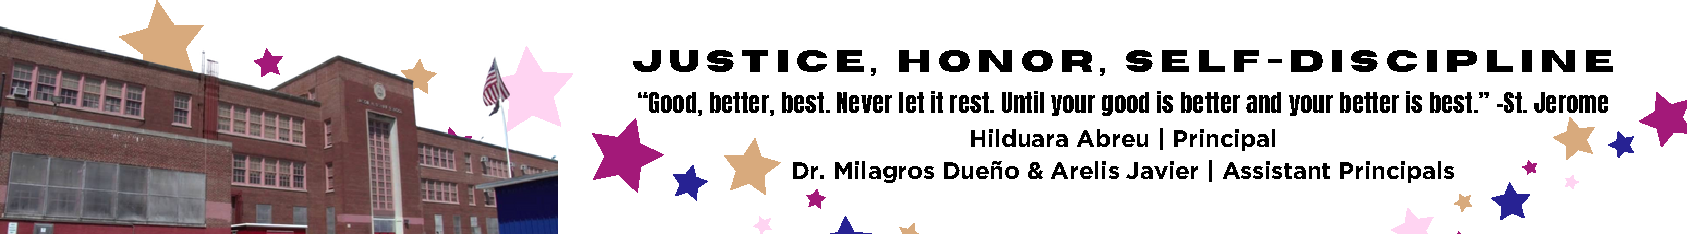
\includegraphics[width=8.8in,height=1.3in]{logo-1}}\end{picture}}
\fancyhead[C]{\setlength{\unitlength}{1in}\begin{picture}(5,0)\put(-1.9,-0.5){
\includegraphics[width=8.9in,height=1.3in]{logo-2}}\end{picture}}
\fancyhead[R]{\thepage}
\pagenumbering{gobble}

\begin{document}
\newpage
\vspace*{0.5cm}
\emph{\textbf{Subject: Welcome to February, 2025 at PS 192: The School of Joyful Learning!}}

Dear PS192 Families,

I hope this letter finds you well and staying warm as we move through February! This month brings with it a sense of love, connection, and a well-deserved break for our students.

As we celebrate Valentine’s Day, let’s take a moment to appreciate the kindness and friendships that make our school community so special. Shortly after, we’ll have our Mid-Winter Recess from February 17th to February 21st. This is a wonderful opportunity for families to enjoy quality time together. If you’re looking for ways to keep your children engaged, I encourage you to explore the city’s incredible museums, visit the Public Library for events or some cozy reading time, or take advantage of the library’s many online resources.

At PS 192, we have a full schedule both before and after the break. Here are some important dates to keep in mind:

\begin{itemize}
\item 📌 3K, Pre-K, Kindergarten, and Middle School Applications for the 2025-2026 school year are due
\item 📌 Coffee with the Principal \& Parent Association Meeting + Valentine’s Day Celebration – February 14th, 8:00 AM in the Gym
\item 📌 Graduation Meeting – February 27th
\begin{itemize}
\item Pre-K \& Kindergarten: 2:30 PM - 3:00 PM
\item 5th Grade: 3:20 PM - 4:00 PM (Library)
\end{itemize}
\end{itemize}

I hope you all have a restful and joyful Mid-Winter Recess filled with love and laughter. Happy Valentine’s Day!

With Justice, Honor, and Self-Discipline,


\includegraphics[width=0.2\textwidth]{hil_signature}

\textbf{Hilduara Abreu, Principal}

\textbf{The School of Joyful Learning!}

\href{www.ps192.org}{www.ps192.org}

\newpage

\fancyfoot[C]{\setlength{\unitlength}{1in}\begin{picture}(5,0)\put(-1.8,-0.5){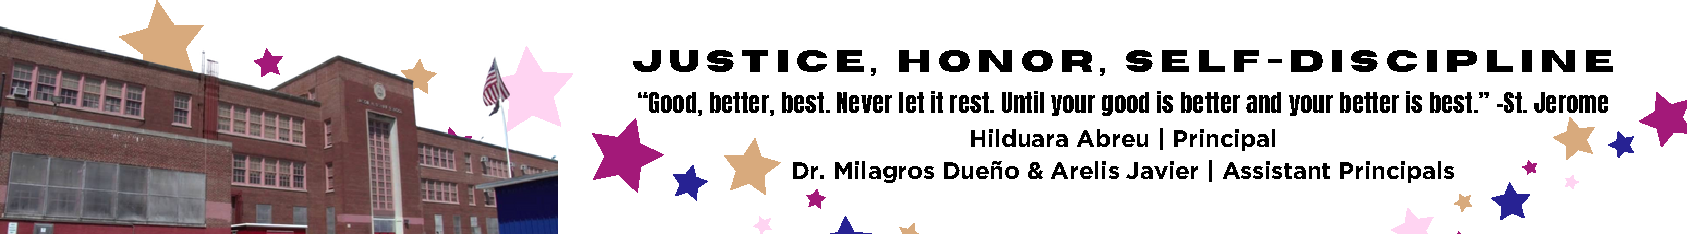
\includegraphics[width=8.8in,height=1.3in]{logo-1}}\end{picture}}
\fancyhead[C]{\setlength{\unitlength}{1in}\begin{picture}(5,0)\put(-1.9,-0.5){
\includegraphics[width=8.9in,height=1.3in]{logo-2}}\end{picture}}
\fancyhead[R]{\thepage}
\pagenumbering{gobble}

\begin{document}
\newpage
\vspace*{0.1cm}
\emph{\textbf{Asunto: Bienvenidos a febrero de 2025 en PS 192: ¡La Escuela del Aprendizaje Alegre!}}

\textbf{Estimados padres y tutores},

\textbf{Espero que esta carta los encuentre bien y abrigados mientras avanzamos en febrero.} ¡Este mes trae consigo un sentido de amor, conexión y un merecido descanso para nuestros estudiantes!

Al celebrar el \textbf{Día de San Valentín}, tomémonos un momento para apreciar la bondad y las amistades que hacen que nuestra comunidad escolar sea tan especial. Poco después, tendremos nuestro \textbf{Receso de Invierno} del \textbf{17 al 21 de febrero}. Esta es una maravillosa oportunidad para que las familias disfruten de tiempo de calidad juntas. Si buscan actividades para mantener a sus hijos comprometidos, los animo a explorar los increíbles \textbf{\textbf{museos de la ciudad}}, visitar la \textbf{\textbf{Biblioteca Pública}} para eventos o un rato acogedor de lectura, o aprovechar los muchos \textbf{\textbf{recursos en línea}} de la biblioteca.

En \textbf{PS 192}, tenemos un calendario lleno tanto antes como después del receso. Aquí hay algunas fechas importantes para recordar:

\begin{itemize}
\item 📌 \textbf{Fecha límite para las solicitudes de 3K, Pre-K, Kindergarten y Secundaria para el año escolar 2025-2026}
\item 📌 \textbf{Café con la Directora y Reunión de la Asociación de Padres + Celebración del Día de San Valentín} – \textbf{14 de febrero, 8:00 AM en el gimnasio}
\item 📌 \textbf{Reunión de Graduación – 27 de febrero}

🔹 \textbf{Pre-K y Kindergarten:} 2:30 PM - 3:00 PM
🔹 \textbf{5 grado:} 3:20 PM - 4:00 PM (Biblioteca)
\end{itemize}

Espero que todos tengan un \textbf{receso de invierno relajante y lleno de amor y alegría}. ¡*Feliz Día de San Valentín!* 💖🎉

Con justicia, honor y autodisciplina,


\includegraphics[width=0.2\textwidth]{hil_signature}

\textbf{Hilduara Abreu, Principal}

La escuela del aprendizaje allegro!

\href{www.ps192.org}{www.ps192.org}
\end{document}
